\begin{abstract}
Cumacea (crustaceans: Peracarida) are vital indicators of benthic health in marine ecosystems. This study investigated the influence of ecological and geographic parameters on their genetic variability in the North Atlantic, focusing on Icelandic waters. We analyzed mitochondrial 16S rRNA gene sequences from 62 cumaceans specimens collected across varying depths. We used \textit{aPhyloGeo} software to correlate these sequences with geographic, environmental, and climatic data encompassing latitude at the start of sampling (decimal degree) (see Figure \ref{fig:fig1}a), water temperature ($^\circ$C) (see Figure \ref{fig:fig1}e) as well as O\textsubscript{2} concentration (mg/L) (see Figure \ref{fig:fig1}f), depth (m) at the start of sampling (see Figure \ref{fig:fig1}c), and other relevant factors.

Our analyses revealed variability in geographic and environmental parameters, such as longitude at the start of sampling (decimal degree), depth (m) at the beginning of sampling, as well as water temperature ($^\circ$C) and O\textsubscript{2} concentration (mg/L) (see Figures \ref{fig:fig1}b, \ref{fig:fig1}c, \ref{fig:fig1}e and \ref{fig:fig1}f). Specific genetic sequences correlated with wind speed (m/s) and O\textsubscript{2} concentration (mg/L) (see Figures \ref{fig:fig5}d and \ref{fig:fig6}d), suggesting potential local adaptations to these fluctuating environmental conditions.

These initial findings highlight the need for further exploration to understand the relationships between cumacean's genetics and their environment. This study lays the foundations for establishing correlations between specific regions of the mitochondrial 16S rRNA gene and the characteristics of their habitat. If substantiated, these findings would support the hypothesis of natural selection driving local adaptation of cumacean to environmental gradients in the face of climate change. The \textit{aPhyloGeo} Python package is freely and publicly available on \href{https://github.com/tahiri-lab/aPhyloGeo}{GitHub}, and it is also available on \href{https://pypi.org/project/aphylogeo/}{PyPi}, to facilitate complex analyses.
\end{abstract}

\section{Introduction}\label{introduction}
The vast North Atlantic and subarctic regions, particularly the Icelandic area and its surrounding waters, present ecological interest due to their various water bodies and unique oceanographic as well as hydrographic characteristics \citep{schnurr_composition_2014, meisner_benthic_2014, uhlir_adding_2021}. The latter form {benthic habitats}\footnote{Benthic habitats are areas on the bottom of the ocean or lake, including the sediments and organisms that live there \citep{levin2009ecological}.} and enhance our understanding of deep-sea ecosystems and biodiversity patterns \citep{rogers2007corals, danovaro2008exponential, meisner_benthic_2014, uhlir_adding_2021}. The IceAGE project and its predecessors, BIOFAR and BIOICE, are invaluable data resources for addressing the impacts of climate change and seabed mining \citep{meisner_prefacebiodiversity_2018}. 

The Greenland, Iceland, and Norwegian (GIN) seas, along with the high-latitude North Atlantic's role in global {thermohaline circulation}\footnote{This is a system of ocean currents produced by differences in seawater density, which in turn are determined by temperature (thermo) and salinity (haline) \citep{talley2013closure}.} is vital for deep-sea ventilation as well as renewal \citep{johannessen_relationship_1994} and slowing formation of cold, deep water due to Arctic sea ice loss can impact their regional dynamics and chemistry \citep{meisner_prefacebiodiversity_2018}. Furthermore, there is a growing international interest in deep-sea resource extraction \citep{mengerink_call_2014}, particularly targeting mid-ocean ridges and other active geothermal areas. Like the Reykjanes Ridge, the ridges around Iceland are home to hydrothermal vent sites. Baseline data are crucial for assessing the damage and loss of ecosystem services caused by climate change and mining activities \citep{meisner_prefacebiodiversity_2018}. 

Cumacea, a crustaceans taxon within Peracarida, is an important indicator of marine ecosystem health due to their high susceptibility to environmental fluctuations \citep{stransky_diversity_2010} and their contribution to benthic foods webs \citep{rehm2009cumacea}. Their diversity and abundance are likely to represent local environments' quality, making them crucial for ecological monitoring studies \citep{hessler1967faunal}. However, the evolutionary history and dynamics of deep-sea benthic invertebrates in the North Atlantic persist in being less studied than those in rocky intertidal environments. Understanding these deep-sea organisms' genetic distribution and demography is fundamental for predicting their response to climate change and range expansion \citep{jennings_phylogeographic_2014}.   

In response to the current climate emergency, we aim to analyze the influence of geographic, environmental, and climatic parameters on the cumacean genetics. As stipulated in the hypothesis of Darwin, individuals best adapted to their environment are likely to survive, reproduce, and evolve. The objective of this study is to deepen and strengthen the natural selection hypothesis by examining whether there is a correlation between the genetic information of the mitochondrial 16S rRNA gene region of cumacean species sampled and the properties of their habitats. If applicable, we'll determine which of our environmental attributes correlates best with a specific genetic sequence (i.e. window) and identify the protein associated with that gene. Our approach includes a comparative study to validate different {phylogeographic models}\footnote{Phylogeographic models are computational tools that analyze the relationships between the genetic structures of populations and their geographical distributions. By incorporating environmental variables, we can interpret how the latter impacts the genetic distribution of cumacean species.} by comparing them with geographic parameters and factors found inside (environmental) and outside (climatic) the waters of the North Atlantic seas around Iceland. Additionally, we will update a Python package (currently in beta), called \textit{aPhyloGeo}, to simplify these complex analyses.

This paper is organized as follows: Section \autoref{related-works} reviews related work on the biodiversity and biogeography of deep-sea benthic invertebrates. Section \autoref{materials-methods} details the materials and methods used in this study, including sampling procedures, genetic analyses, and geographic and ecological data collection. Section \autoref{metrics} describes the metrics used to evaluate phylogeographic models. Section \autoref{results} presents the results of our analyses. Finally, Section \autoref{conclusion} summarizes our findings and discusses their implications for future research and conservation efforts.

\section{Related Works}\label{related-works}
Assessing and quantifying the biodiversity of deep-sea benthic invertebrates has become an increasingly critical issue since it was discovered that their richness can be underestimated \citep{grassle1992deep}. Subsequent research has highlighted the importance of developing and implementing large-scale distribution models for these organisms to understand their diversity across their ecological and evolutionary origins \citep{rex1997large}. This is why recent efforts have been devoted to mapping, managing, and studying the seabed. Cutting-edge technologies, such as acoustic detection, are being used to improve our knowledge of the complexity of benthic ecosystems \citep{brown2011benthic}. Therefore, an approach that integrates their genetic and environmental characteristics would provide a better understanding of how environmental factors influence the genetic differences, distribution, biodiversity, and resilience of deep-sea benthic organisms \citep{etter1990population, vrijenhoek2009cryptic}.

However, studies have highlighted the complexity of the relationships between genetics and the environment, influenced by genotype-environment interaction and natural selection factors, making it challenging to identify clear causal relationships \citep{balkenhol_identifying_2009}. Distinguishing between the direct and indirect effects of the environment on genetics can be just as complex \citep{manel_perspectives_2010, balkenhol_landscape_2019}. The methods available to measure genetic and environmental characteristics and logistical constraints often limit the scale of studies \citep{manel_perspectives_2010, shafer_widespread_2013}. This can explain why research into cumacean’s environment and genetics has been little explored, even though they remain essential for understanding how these deep-sea invertebrates adapt to fluctuating environmental conditions.


\section{Our Contribution}

Our study investigates the genetic variation of cumacean populations in the face of environmental fluctuations. We aim to identify the genetic region with the highest mutation rate, its correlation with geographic, climatic, and environmental distribution patterns, and the potential protein associated with it. Through robust analytical methods, including dissimilarity calculations and phylogenetic reconstruction, we provide insights into the genetic adaptation of marine crustaceans. Our findings contribute to understanding evolutionary dynamics in marine ecosystems. In addition, our genetic and environmental information highlights critical habitats and regions of high conservation interest, which can be considered for establishing marine protected areas. Finally, our study initiates further research on other invertebrate species and in different geographical regions. By extending the research and analysis to various environments and taxonomic groups, scientists will gain a broader picture of the adaptation and resilience of marine invertebrates to climate change.

\section{Materials and Methods}\label{materials-methods}
This section will describe our data and outline the main steps used in data preprocessing and the software \textit{aPhyloGeo}. 

\subsection{Description of the data}
The study area was located in a northern region of the North Atlantic, including the Icelandic Sea, the Denmark Strait, and the Norwegian Sea. The specimens examined were gathered during the IceAGE project (Icelandic marine Animals: Genetic and Ecology; Cruise ship M85/3 in 2011), which investigated the deep continental slopes and abyssal waters around Iceland \citep{meisner_prefacebiodiversity_2018}. The sampling period for the specimens included was from August 30 to September 22, 2011, and they were collected at depths ranging from 316 to 2568 m. Information about the sampling plan, sample processing, the steps of DNA extraction, PCR amplification, sequencing, and the extracted and aligned DNA sequences are available in the article by \citep{uhlir_adding_2021}.

\subsection{Data pre-processing}
We used data from the IceAGE project and related data from the BOLD Systems database, both accessible through the article by \citep{uhlir_adding_2021}. Given these databases' enormous scope of attributes, we selectively reduced the number of attributes and samples. Specifically, we omitted attributes that were not relevant to the context of this study, were entirely or nearly invariable (non-numerical data), or had abundant missing data (>95\%). From the IceAGE project dataset, we considered 62 specimens out of the 495 available. Subsequently, we calculated the variance for each of the selected numeric attributes to eliminate those with zero or low variance (cut-off ≤ 0.1). Equation \ref{variance} provides the formula for variance used in this study.

\begin{equation}\label{variance}
    S^2 = \frac{\sum_{i=1}^{n} (x_i - \bar{x})^2}{n-1}
\end{equation}

where $S^2$ is the sample variance, $x_i$ represents each value in the dataset, $\bar{x}$ the average of all values in the dataset, and $n$ the number of values in the dataset.

Only salinity was removed from the previously selected numerical attributes ($S^2 = 0.02146629$). This selection of attributes and data resulted in a data table containing 62 rows ($n=62$) and 18 columns (number of attributes). 

From the IceAGE database, 14 attributes were selected. These consist of the geographical coordinates such as: 

\begin{itemize}
\item The latitude and longitude taken at the beginning (see Figures \ref{fig:fig1}a and \ref{fig:fig1}b) and at the end of sampling, both on decimal degree (DD).
\item These geographic data are divided into five sectors across the seas around Iceland: the Denmark Strait ($n=28$), the Iceland Basin ($n=15$), the Irminger Basin ($n=12$), the Norwegian Sea ($n=4$), and the Norwegian Basin ($n=3$). 
\end{itemize}

Concerning the environmental attributes, we included:
\begin{itemize}
\item The depth (m) at the beginning (see Figure \ref{fig:fig1}c) and end of sampling as well as the temperature ($^\circ$C) (see Figure \ref{fig:fig1}e) and O\textsubscript{2} concentration (mg/L) (see Figure \ref{fig:fig1}f) of the water depending on the depth at which the specimens were sampled. 
\item The sedimentary characteristics of the sampling sites, which influence the distribution of Cumacea \citep{uhlir_adding_2021}. In this study, they fall into six categories: mud ($n=30$), sandy mud ($n=15$), sand ($n=9$), forams ($n=3$), muddy sand ($n=3$), and gravel ($n=2$).
\end{itemize}

Climatic parameters such as: 
\begin{itemize}
\item Wind speed (m/s) (see Figure \ref{fig:fig1}d) and wind direction at the beginning and end of sampling were also included, given the contribution of wind to the restructuring of the benthic ecosystem through water transport \citep{waga_recent_2020,saeedi_environmental_2022}. The wind direction at the start of sampling consists of six orientations: South-West ($n=22$), South ($n=15$), North-East ($n=9$), South-South-East ($n=9$), North-West ($n=5$), and East ($n=2$); while the one at the end of sampling is made up of seven orientations: South ($n=15$), South-West ($n=15$), North-East ($n=9$), West-South-West ($n=7$), South-East ($n=6$), North-North-West ($n=5$), South-South-East ($n=3$), and East ($n=2$). 
\end{itemize}

In the BOLD Systems database, taxonomic ranks such as: 
\begin{itemize}
\item Family, genus, and species of the sampled cumacean were integrated in our data. These are composed of seven families: Diastylidae ($n=21$), Lampropidae ($n=13$), Leuconidae ($n=12$), Nannastacidae ($n=7$), Bodotriidae ($n=4$), Ceratocumatidae ($n=3$), and Pseudocumatidae ($n=2$). A total of 21 species of cumacean are found in our sample (see Figure \ref{fig:fig2}).
\end{itemize}

It should be noted that some specimens were identified only to genus (one specimen) or to family (five specimens) in our sample.
 
The habitat and water mass of the sampling points are the only attributes that were taken directly via Table 1 of \citep{uhlir_adding_2021}. Thus, the definitions of water bodies described by \citep{hansen_north_2000, brix2010distribution, ostmann_marine_2014} were used as a reference for the GIN seas around Iceland: Arctic Polar Water (APW, $n=15$), Iceland Sea Overflow Water (ISOW, $n=15$), North Atlantic Water (NAW, $n=9$), Arctic Polar Water/Norwegian Sea Arctic Intermediate Water (APW/NSAIW, $n=7$), warm Norwegian Sea Deep Water (NSDWw, $n=8$), Labrador Sea Water (LSW, $n=3$), cold Norwegian Sea Deep Water (NSDWc, $n=3$), and Norwegian Sea Arctic Intermediate Water (NSAIW, $n=2$) (see Figure \ref{fig:fig3}). In terms of habitat, we considered the three categories used in \citep{uhlir_adding_2021}: deep sea ($n=38$), shelf ($n=15$), and slope ($n=9$) (see Figure \ref{fig:fig4}).

To better interpret the relation and evolutionary responses of benthic species, genetic data are needed \citep{wilson_speciation_1987, uhlir_adding_2021}. Thus, the aligned DNA sequence of the mitochondrial 16S rRNA gene region of each of the samples was included in our analyses. This region is not only standard in phylogeny and phylogeography studies \citep{hugenholtz1998impact}, but is sufficiently conserved over time to ensure exact alignments between different species or populations \citep{saccone1999evolutionary}. We considered 62 of the 306 aligned DNA sequences that were used for phylogenetic analyses by \citep{uhlir_adding_2021}. Since some of the specimens in our sample have their DNA sequence duplicated, or even quadrupled with a difference of one to two nucleotides, we considered the longest-aligned DNA sequence of each specimen. 

Figures \ref{fig:fig1}, \ref{fig:fig2}, \ref{fig:fig5} and \ref{fig:fig6} were made using Python 3.11, while Figures \ref{fig:fig3} and \ref{fig:fig4} were made using RStudio Desktop 4.3.2.

\subsection{\textit{aPhyloGeo} software}

We used the cross-platform Python software \textit{aPhyloGeo} for our phylogeographic analyses, designed to analyze phylogenetic trees using ecological and geographic parameters. Developed by My-Linh Luu, Georges Marceau, David Beauchemin, and Nadia Tahiri, \textit{aPhyloGeo} offers tools to study correlations between species genetics and habitat characteristics, enabling us to understand the evolution of species under different environmental conditions. This software was chosen for our analysis because, to our knowledge, it is the first phylogeographic tool to correlate species genetics with climatic, environmental, and geographical attributes, which is what we aim to achieve with our study. The \textit{aPhyloGeo} Python package is freely and publicly available on \href{https://github.com/tahiri-lab/aPhyloGeo}{GitHub}, and it is also available on \href{https://pypi.org/project/aphylogeo/}{PyPi}, to facilitate complicated analyses. The software process takes three main steps (see \autoref{lst:main}).


%\autoref{lst:main}.
\begin{lstlisting}[label=lst:main,language=Python,caption=Main script for tutorial using the aPhyloGeo package.]
if __name__ == "__main__":

    # Load parameters
    Params.load_from_file()
    # Load the sequence file
    sequenceFile = utils.loadSequenceFile(Params.reference_gene_filepath)
    # Create an AlignSequences object
    align_sequence = AlignSequences(sequenceFile)

    # Load climatic data 
    climatic_data = pd.read_csv(Params.file_name)

    # Perform the alignment of sequences
    alignments = align_sequence.align()

    # Generate genetic trees
    geneticTrees = utils.geneticPipeline(alignments.msa)
    
    # Create a GeneticTrees object
    trees = GeneticTrees(trees_dict=geneticTrees, 
                        format="newick")
   
    # Generate climatic trees
    climaticTrees = utils.climaticPipeline(climatic_data)
    
    # Filter the results
    utils.filterResults(climaticTrees, 
                        geneticTrees, 
                        climatic_data)

\end{lstlisting}

\begin{enumerate}
\item \textbf{The first step} is to collect cumacean DNA sequences of sufficient quality for the requirements of our results \citep{koshkarov_phylogeography_2022}. A total of 62 cumacean samples were selected to represent 62 sequences of the gene mitochondrial 16S rRNA. Subsequently, we included two climatic factors, namely the wind speed (m/s) at the beginning and end of the sampling. We also included four environmental factors, such as the depth (m) of sample collection at the beginning and end of sampling, the temperature ($^\circ$C), and O\textsubscript{2} concentration (mg/L) of the water. Finally, we have integrated four geographical parameters, including the latitude (DD) and longitude (DD) at the beginning and end of sampling.

\item \textbf{In the second step}, the trees were generated with environmental, geographical, climatic, and genetic data. Concerning the geographic parameters, we calculated the dissimilarity between each data pair from different geographic conditions, producing a symmetric square matrix. The neighbor-joining algorithm was used to design the geographic tree from this matrix. The same approach was applied to environmental, climatic, and genetic data. A method involving iterative phylogenetic reconstruction was employed to construct gene trees based on 62 sequences of mitochondrial 16S rRNA, considering only the data within a range that moves along the alignment. This displacement can vary depending on the steps and window size the user sets (their length is defined by the number of base pairs (bp)) \citep{koshkarov_phylogeography_2022}.

\item \textbf{In the third step}, the phylogenetic trees built in each sliding window are compared to environmental, climatic and geographical parameters using the Robinson-Foulds (RF) distance \citep{robinson_comparison_1981, koshkarov_phylogeography_2022}, the normalized Robinson-Foulds distance, the Euclidean distance, and the Least-Squares distance. These contribute to our understanding of similarities and dissimilarities between genetic sequences of organisms. The distance was normalized by $2n-6$, where $n$ represents the number of taxa. The approach also took bootstrapping into account. Using the sliding window allowed detailed identification of regions with high genetic mutation rates \citep{koshkarov_phylogeography_2022}.
\end{enumerate}

\section{Metrics}\label{metrics}
The following section presents a more concise version of the formulas mentioned in the third step of the preceding section:

\subsection{Robinson-Foulds Distance (RF distance)}\label{RF}
The Robinson-Foulds distance measures the dissimilarity between two phylogenetic trees by counting the pairs of clades present in one tree but absent in the other. It is commonly used to quantify topological differences between two phylogenetic trees (see Equation \eqref{eq:rf} and \autoref{lst:robinsonFoulds}).

\begin{equation}\label{eq:rf}
    \text{RF}(T_1, T_2) = | \Sigma(T_1) \Delta \Sigma(T_2) |
\end{equation}

where $\Sigma(T_1)$ and $\Sigma(T_2)$ are the sets of splits in trees $T_1$ and $T_2$.

%\autoref{lst:robinsonFoulds}.
\begin{lstlisting}[label=lst:robinsonFoulds,language=Python,caption=Python script for calculating the Robinson-Foulds distance using the ete3 package in the aPhyloGeo package.]
    def robinsonFoulds(tree1, tree2):
        rf = 0
        tree1_newick = ete3.Tree(tree1.format("newick"), format=1)
        tree2_newick = ete3.Tree(tree2.format("newick"), format=1)

        rf, rf_max, common_leaves = tree1_newick.robinson_foulds(tree2_newick, 
                                                                 unrooted_trees=True)
        if len(common_leaves) == 0:
            rf = 0

        return rf, rf / rf_max
\end{lstlisting}


\subsection{Normalized Robinson-Foulds Distance}\label{RFnorm}
The normalized Robinson-Foulds distance scales the RF distance to account for tree size, allowing a fairer comparison between them and resulting in a value between 0 and 1. In this case, the distance was normalized by $2n-6$, where $n$ represents the number of taxa, to facilitate comparison of relative differences between trees (see Equation \eqref{eq:rf_norm} and \autoref{lst:euclideanDist}).

\begin{equation}\label{eq:rf_norm}
    \text{RF}_{\text{norm}}(T_1, T_2) = \frac{| \Sigma(T_1) \Delta \Sigma(T_2) |}{| \Sigma(T_1) | + | \Sigma(T_2) |}
\end{equation}

\subsection{Euclidean Distance}\label{euclidean}
Euclidean distance measures the length between two points in a multi-dimensional space. It is used to evaluate the overall difference between two nucleotide sequences based on their genetic characteristics (see Equation \eqref{eq:euclidean} and \autoref{lst:euclideanDist}).

For points $\mathbf{p} = (p_1, \ldots, p_n)$ and $\mathbf{q} = (q_1, \ldots, q_n)$:

\begin{equation}\label{eq:euclidean}
    d_{\text{Euclidean}}(\mathbf{p}, \mathbf{q}) = \sqrt{\sum_{i=1}^{n} (p_i - q_i)^2}
\end{equation}

%\autoref{lst:euclideanDist}.
\begin{lstlisting}[label=lst:euclideanDist,language=Python,caption=Python script for calculating the Euclidean distance using the ete3 package in the aPhyloGeo package]
    def euclideanDist(tree1, tree2):
        
        tns = dendropy.TaxonNamespace()
        
        tree1_tc = dendropy.Tree.get(data=tree1.format("newick"), 
                                     schema="newick", 
                                     taxon_namespace=tns)
                                     
        tree2_tc = dendropy.Tree.get(data=tree2.format("newick"), 
                                     schema="newick", 
                                     taxon_namespace=tns)
                                     
        tree1_tc.encode_bipartitions()
        tree2_tc.encode_bipartitions()

        ed = dendropy.calculate.treecompare.euclidean_distance(tree1_tc, tree2_tc)

        return ed
\end{lstlisting}

\subsection{Least-Squares Distance}\label{LS}
The Least-Squares distance measures differences by considering the sum of the squares of differences between the observed and the estimated values provided by the model. In our context, it quantifies the overall dissimilarity between phylogenetic trees constructed from genetic sequences and ecoclimatic and geographical features (see Equation \eqref{eq:ls} and \autoref{lst:LeastSquare}).

For observed values $y_i$ and estimated values $\hat{y}_i$:

\begin{equation}\label{eq:ls}
    d_{\text{LS}} = \sum_{i=1}^{n} (y_i - \hat{y}_i)^2
\end{equation}

These formulas succinctly describe the methods used to measure distances and dissimilarities in various contexts.

%\autoref{lst:LeastSquare}.
\begin{lstlisting}[label=lst:LeastSquare, language=Python, caption=Python script for calculating the Least-Square distance using the ete3 package in the aPhyloGeo package]
def least_square(tree1, tree2):
    ls = 0.0
    leaves = tree1.get_terminals()

    leaves_name = list(map(lambda x: x.name, leaves))
    for i in leaves_name:
        leaves_name.pop(0)
        for j in leaves_name:
            d1 = tree1.distance(tree1.find_any(i), tree1.find_any(j))
            d2 = tree2.distance(tree2.find_any(i), tree2.find_any(j))
            ls += abs(d1 - d2)
    return ls
\end{lstlisting}

Our phylogeographic study used Robinson-Foulds, normalized Robinson-Foulds, Euclidean, and Least-Squares distances to quantify topological differences between phylogenetic trees and assess dissimilarities between genetic sequences and environmental, geographical, and climatic features, providing a comprehensive analysis of evolutionary dynamics in cumacean populations.

\section{Results}\label{results}

To understand the correlation between cumacean genetics and their habitat, we parameterized the \textit{aPhyloGeo} software as follows: pairwiseAligner, Hamming distance, Wider Fit by elongating with Gap (starAlignment), windows size: 1 nucleotide (nt) and window step: 10 nt. The results of the metrics used (Robinson-Fouls, normalized Robinson, Least-Square and Euclidean distances) were obtained using the functions leastSquare(tree1, tree2), robinsonFoulds(tree1, tree2), euclideanDist(tree1, tree2) from the \textit{aPhyloGeo} software and were organized by the main function (see \autoref{lst:main}). A more detailed analysis is provided in \section*{Supplementary material}.

Violon diagrams presented in Figure \ref{fig:fig1} are used to display summary statistics similar to box plots, showing medians (white dots), interquartile ranges (thickened black bars), and the rest of the distributions (thin black lines), except "extreme" points. Larger areas indicate a higher probability of the variables taking a given value. They illustrate the distribution of geographical (latitude and longitude at the start of sampling (DD)), climatic (wind speed (m/s) at the start of sampling), and environmental (depth (m) at the start of sampling, water temperature ($^\circ$C), and O\textsubscript{2} concentration (mg/L)) data. These diagrams are critical for understanding habitat conditions and highlighting unique habitats that can impact cumacean genetics. 

\begin{figure}[htbp]
    \centering
    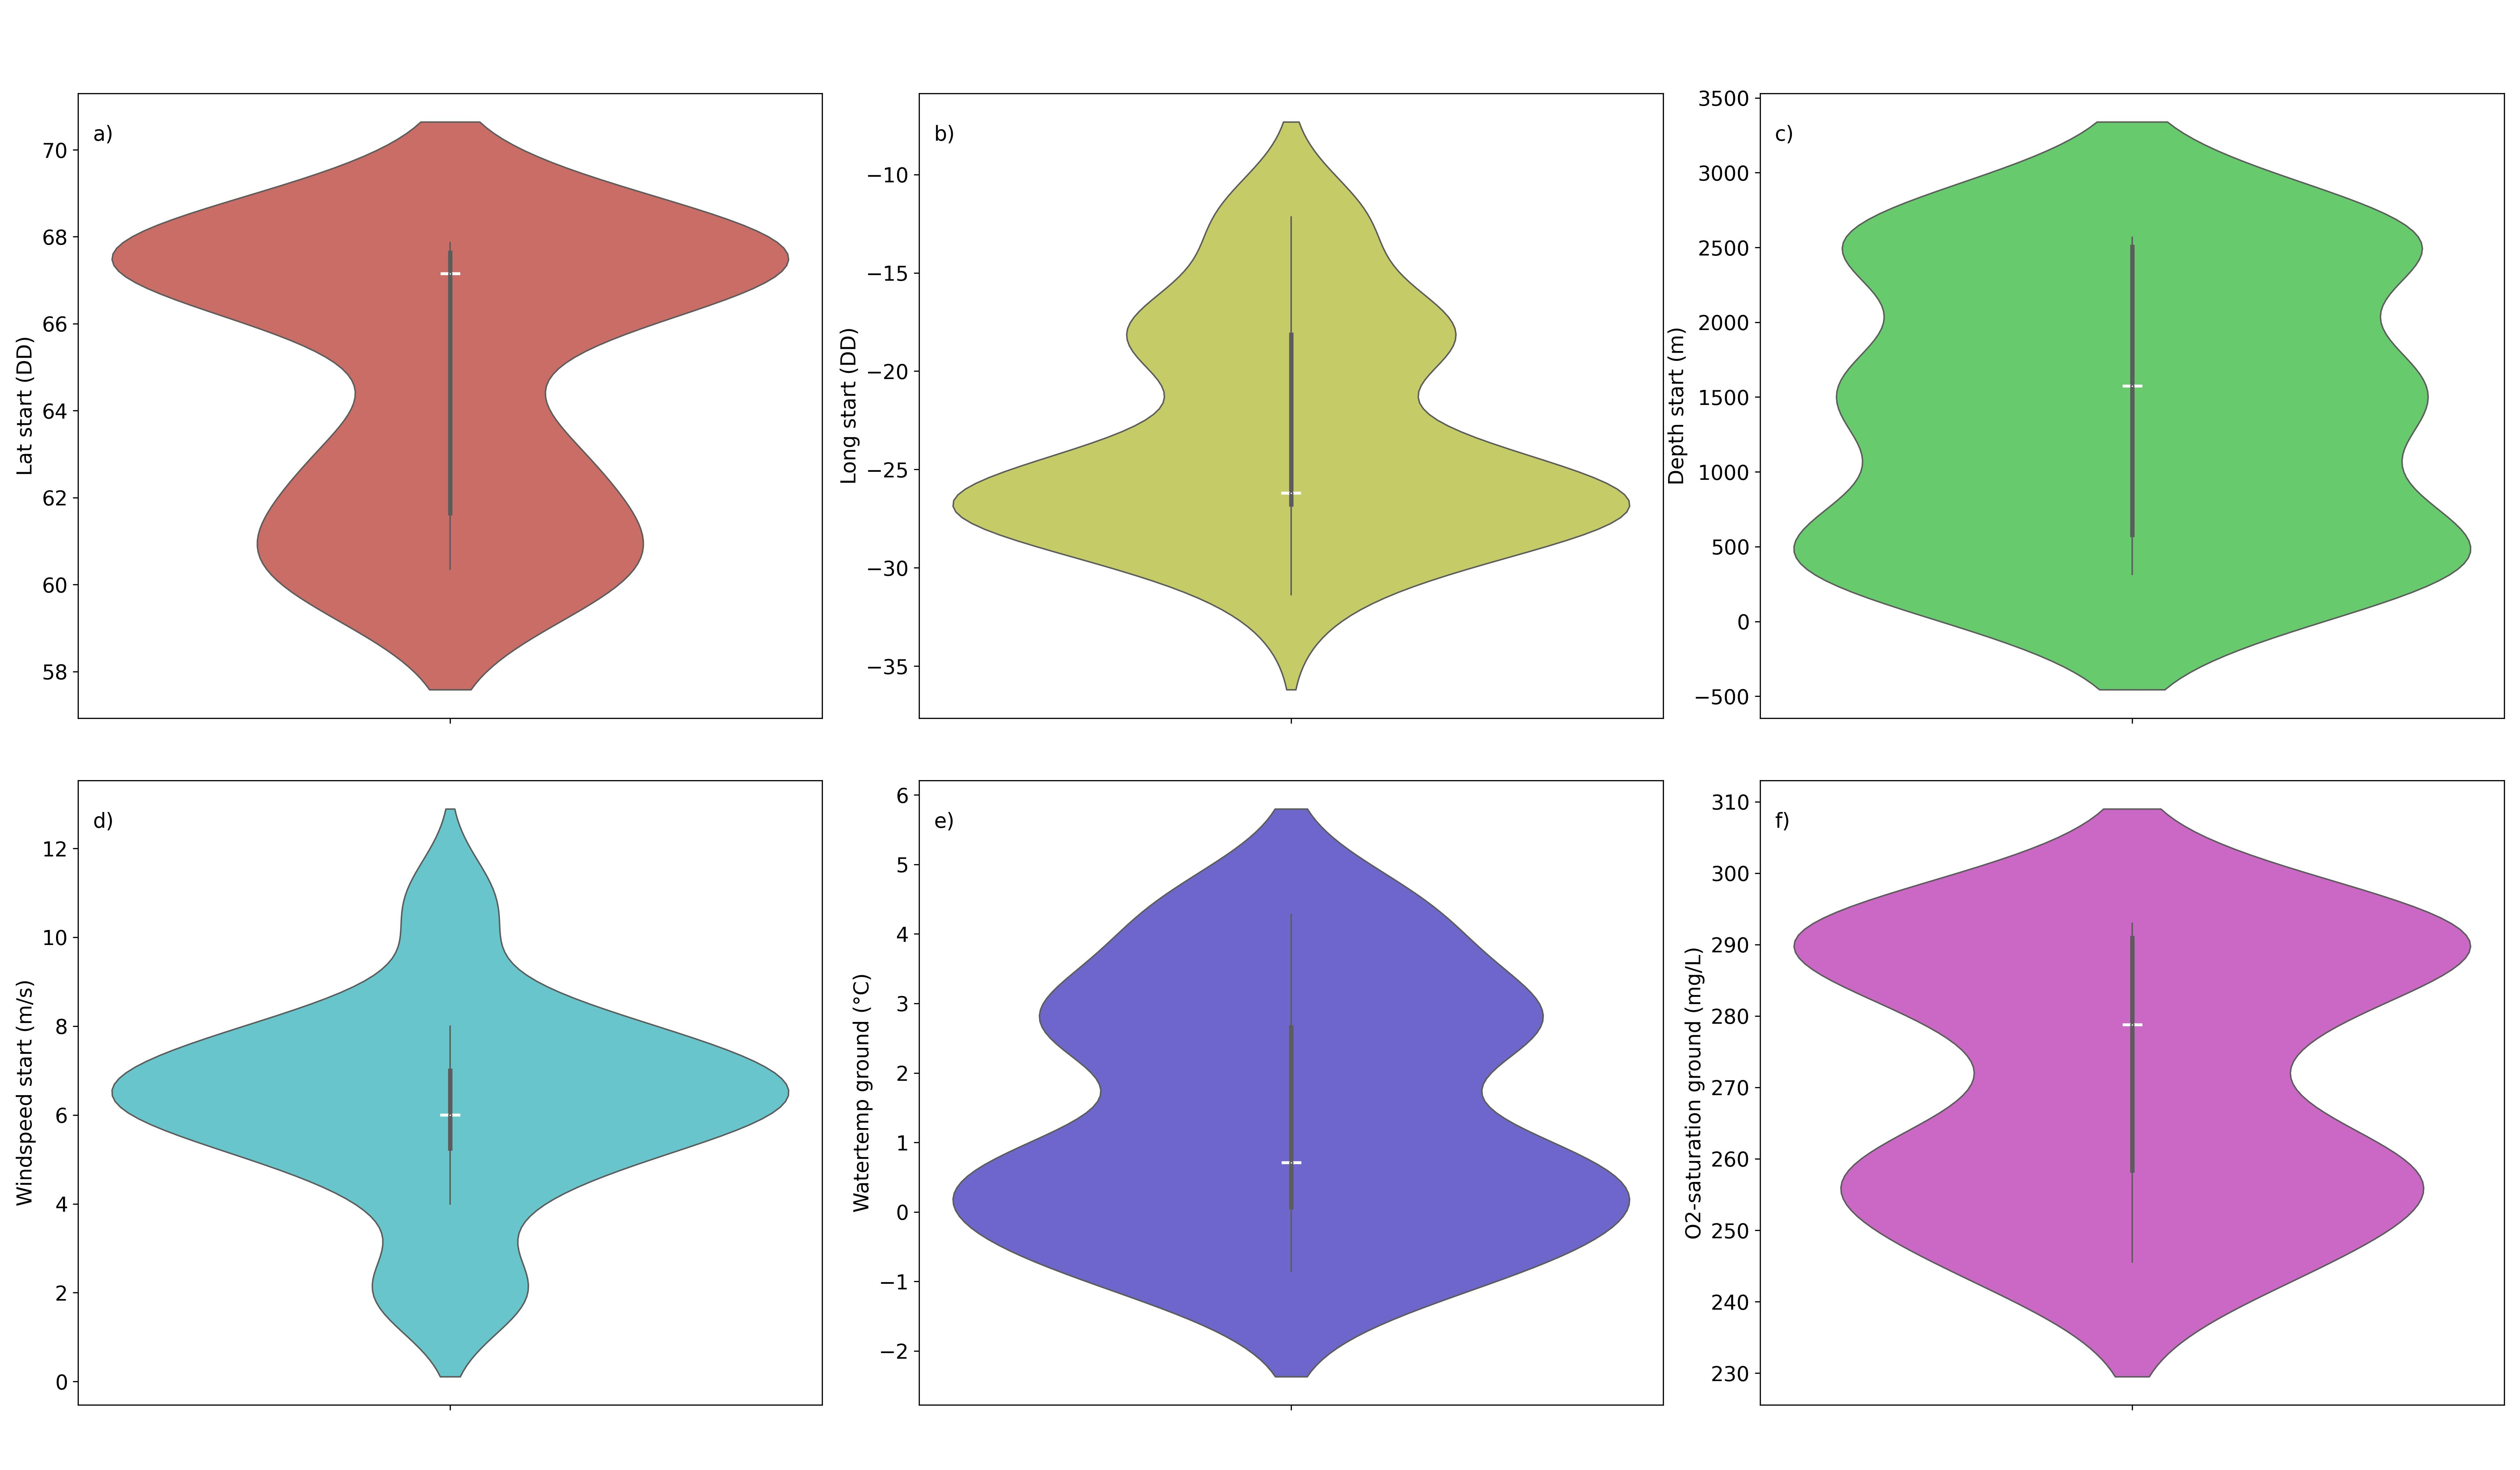
\includegraphics[width=0.7\textwidth]{figure1.jpg}
    \caption{Violin diagrams of six geographical, climatic, and environmental attributes of our sample. a) Latitude (DD) at the start of sampling (red); b) Longitude (DD) at the start of sampling (yellow); c) Depth (m) at the start of sampling (green); d) Wind speed (m/s) at start of sampling (light blue); e) Water temperature ($^\circ$C) according to depth at which the specimens were collected (dark blue); f) O\textsubscript{2} concentration (mg/L) according to depth at which the specimens were sampled (pink). The mean, median, standard deviation (Std Dev), 1st quartile (Q1), and 3rd quartile (Q3) of the dataset for each attribute are shown in the top right-hand corner of each graph. \label{fig:fig1}}
\end{figure}

Our results revealed environmental variability in most cumacean habitat attributes presented in Figure \ref{fig:fig1}. The median of Figure \ref{fig:fig1}a (67.15 DD) is higher than the mean (64.83 DD), indicating a skewed distribution towards lower values. This is also the case for the depth (m) at the start of sampling and water (O\textsubscript{2} concentration (mg/L) (see Figures \ref{fig:fig1}c and \ref{fig:fig1}f). The curve of Figure \ref{fig:fig1}a has an asymmetrical bimodal shape, showing two peaks, suggesting that the samples come from two dominant latitudinal regions at the start of sampling. This could indicate major fluctuations in climatic and environmental conditions in the regions sampled. Similarly, this type of curve is present for the longitude (DD) at the start of sampling, as well as for the temperature ($^\circ$C) and O\textsubscript{2} concentration (mg/L) of the water from which the samples were taken (see Figures \ref{fig:fig1}b, \ref{fig:fig1}e and \ref{fig:fig1}f). 

The median of Figure \ref{fig:fig1}b (-26.21 DD) is lower than the mean (-23.12 DD), indicating an asymmetry on the higher sides, as is the water temperature ($^\circ$C) (see Figure \ref{fig:fig1}e). The standard deviation (5.52 DD) and quartiles Q1 (-26.77 DD) and Q3 (-18.14 DD) indicate a relatively wide range, around the mean (-23.12 DD), of longitude distribution at the start of sampling (-31.356 - -12.162 DD). This suggests a strong environmental gradient, geographical distribution and sample diversity from east to west in the region studied. The standard deviation of Figure \ref{fig:fig1}c is quite high (881.16 m), indicating a great variability in sample collection depths (316 – 2568 m) and giving a more global overview of benthic habitats. This is also confirmed by the quartiles Q1 (579.10 m) and Q3 (2504.70 m). Unlike all the other diagrams of Figure \ref{fig:fig1}, the curve in Figure \ref{fig:fig1}c has a multimodal shape with three prominent peaks, suggesting that the samples were mainly collected and concentrated at three different depths (around 500, 1500, and 2500 m).

The mean (6.26 m/s) and median (6.00 m/s) of Figure \ref{fig:fig1}d are the only ones in Figure \ref{fig:fig1} that are similar, indicating a symmetrical distribution, with a high concentration of data around the median (6.00 m/s). This suggests relatively stable wind conditions (m/s) at the start of sampling. The standard deviation of Figure \ref{fig:fig1}e is relatively high (1.73 $^\circ$C) compared to the mean (1.45 $^\circ$C), indicating a broad range of water temperatures where samples were taken (0.851 – 4.28 $^\circ$C), also supported by quartiles Q1 (0.07 $^\circ$C) and Q3 (2.66 $^\circ$C). This suggests that water temperatures were very different depending on whether or not the sampling zones were close to the water surface, indicating acclimatization of cumaceans to a variety of habitat temperatures. The range of O\textsubscript{2} concentration data (see Figure \ref{fig:fig1}f) shows some variability (245.53 – 292.97 mg/L) in the environmental conditions of the areas sampled, as shown by the standard deviation (18.11 mg/L) and quartiles Q1 (258.39 mg/L) and Q3 (290.90 mg/L). These latest results reflect a diversity of O\textsubscript{2} requirements, with organisms adapted to low O\textsubscript{2} conditions and potentially influenced by the heterogeneity of biogeochemical cycles, such as photosynthesis, respiration, and organic decomposition, which impact dissolved O\textsubscript{2} levels as a function of depth.


\begin{figure}[htbp]
    \centering
    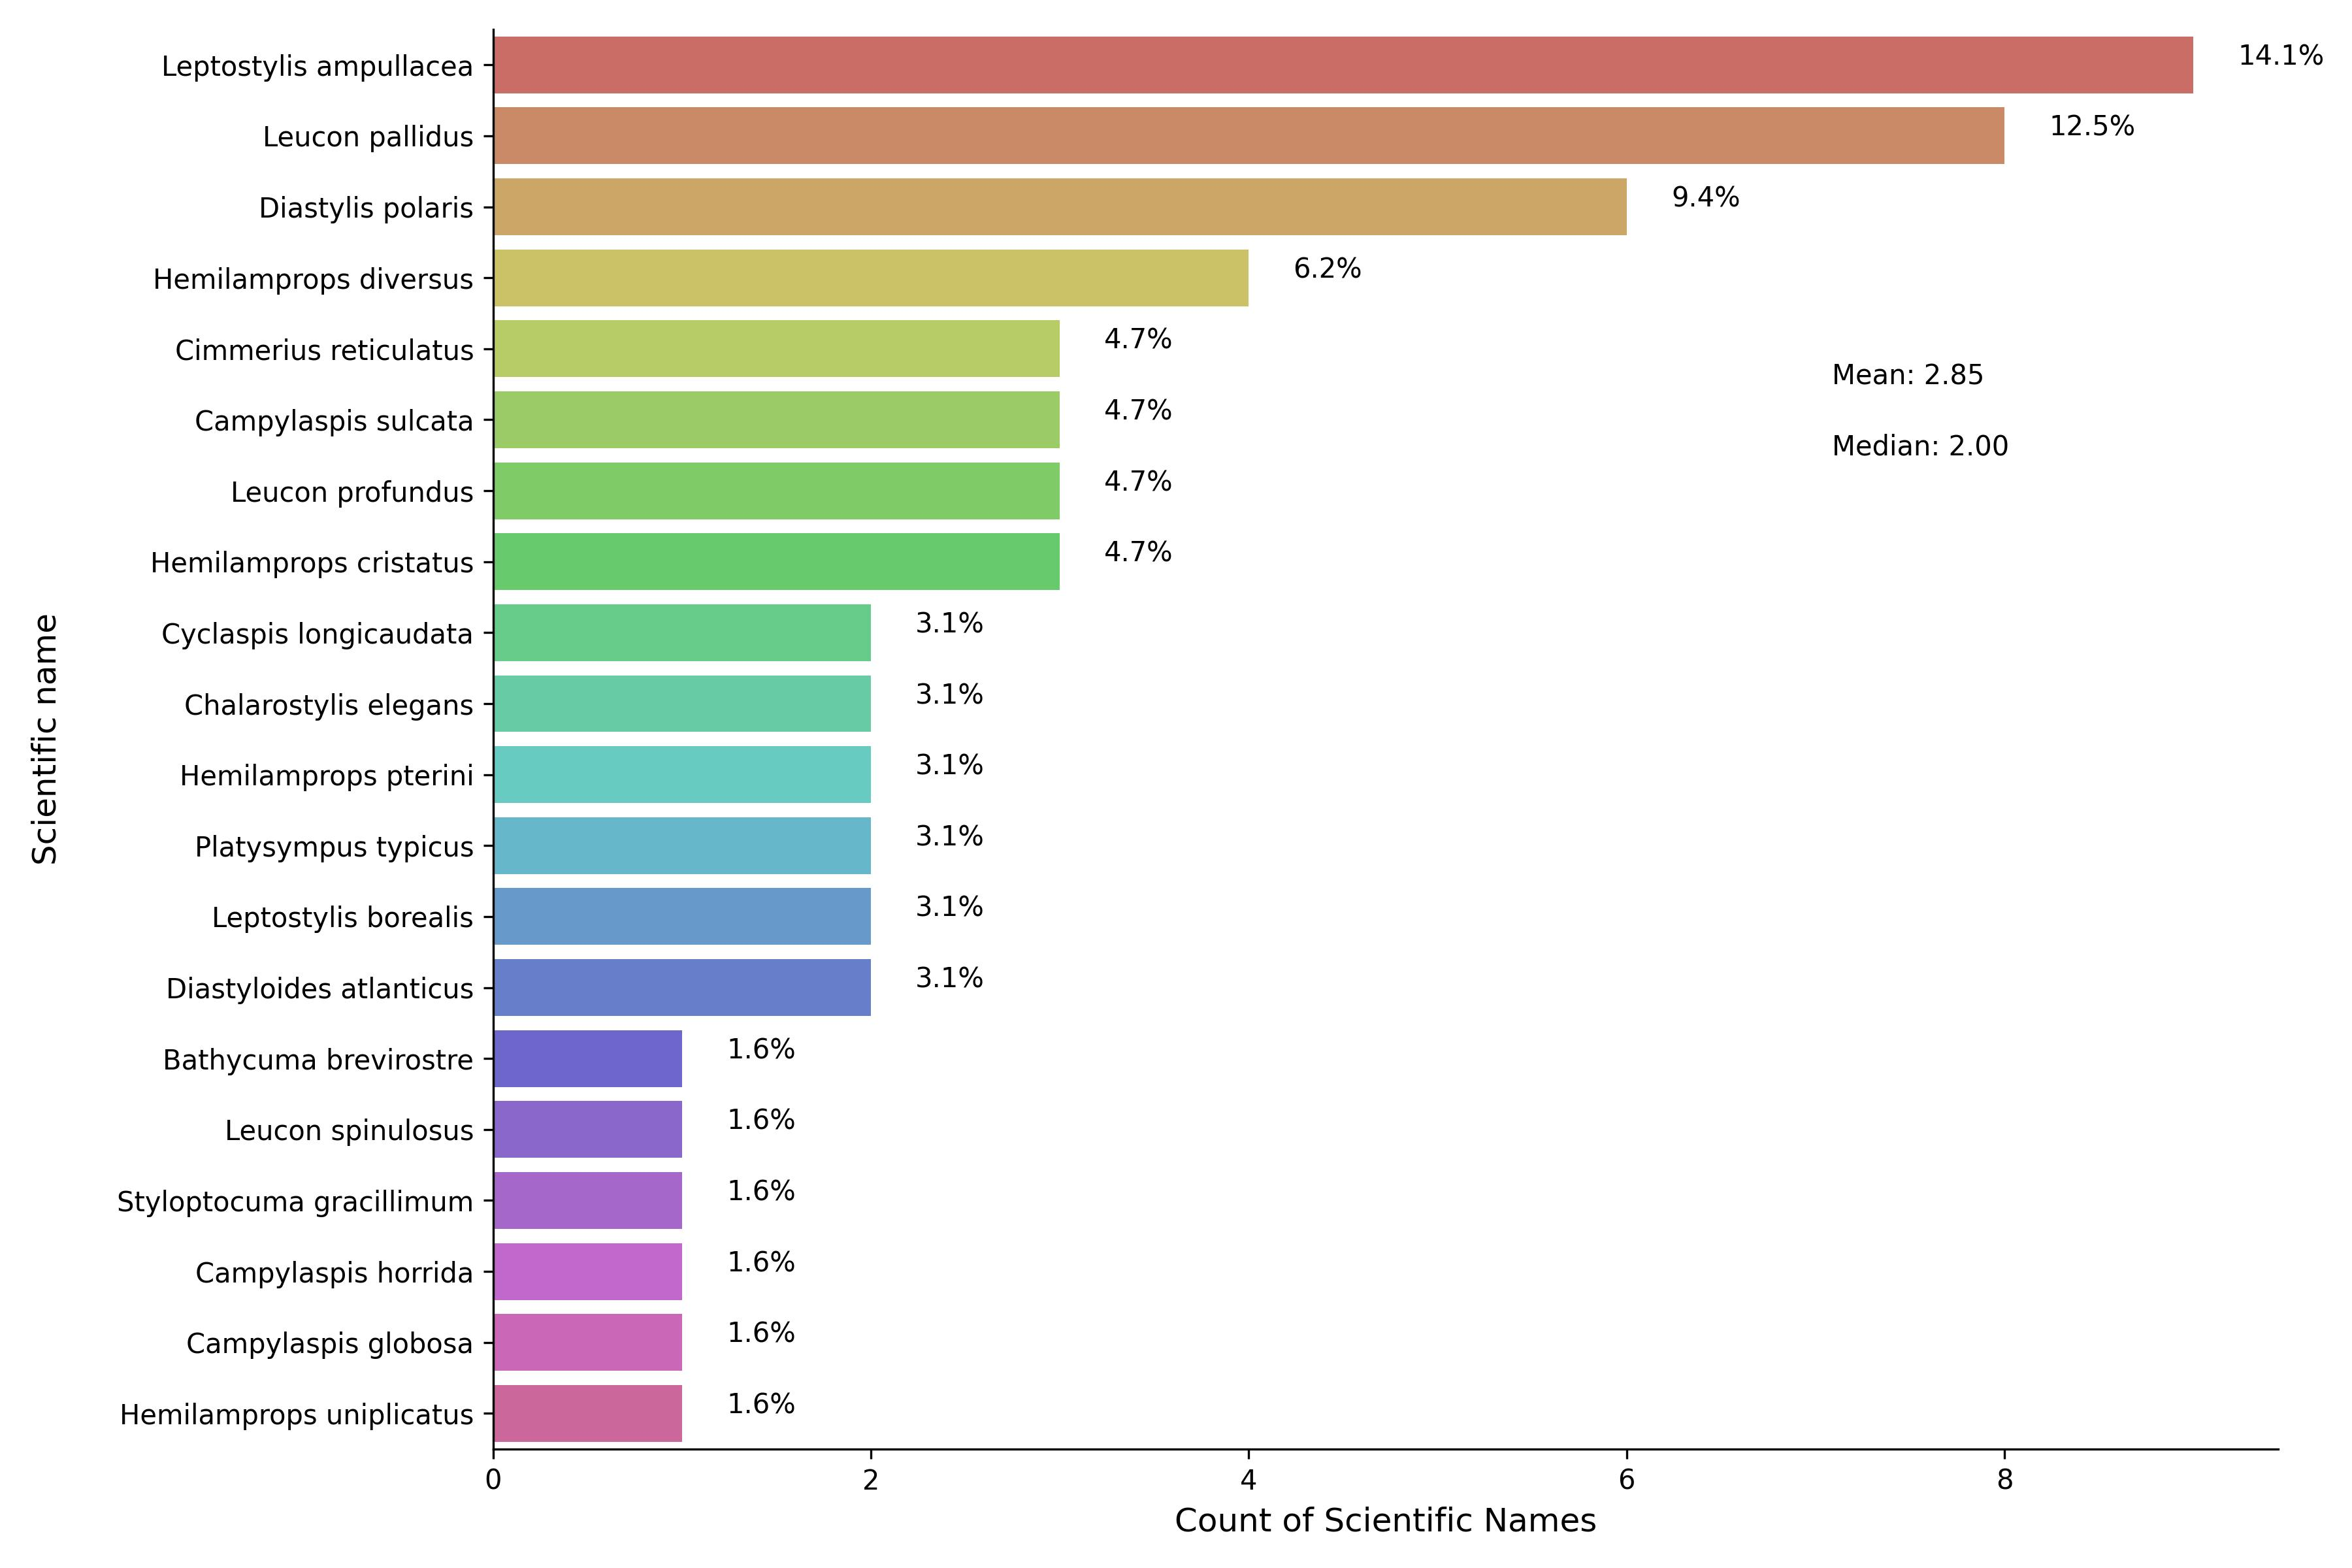
\includegraphics[width=0.7\textwidth]{figure2.jpg}
    \caption{Distribution of cumacean species frequency. This histogram shows the frequency distribution of cumacean species found in our sample. The bars represent the number of individuals for each species. The percentages (\%) displayed above the bars indicate the relative abundance of each species in the total sample. The mean and median values of the frequency distribution are shown in the top right-hand corner of the histogram. \label{fig:fig2}}
\end{figure}

The distribution and diversity of the different cumacean species found in our sample are presented in Figure \ref{fig:fig2}. It helps in visualizing the most represented species (\emph{Leptostylis ampullacea}, 14.1\%; \emph{Leucon pallidus}, 12.5\%) and the less represented species (\emph{Bathycuma brevirostre}, \emph{Leucon spinulosus}, \emph{Styloptocuma gracillimum}, \emph{Campylaspis horrida}, \emph{Campylaspis globosa}, and \emph{Hemilamprops uniplicatus}; all 1.6\%), suggesting variations in sampling, particular ecological forces that favor or limit certain species, or that certain species have a restricted ecological niche. In contrast to the lesser represented species, dominant species may have particular adaptive traits that contribute to their exploitation of food, their interspecific competition, or their resistance to changing environmental conditions.

\begin{figure}[htbp]
    \centering
    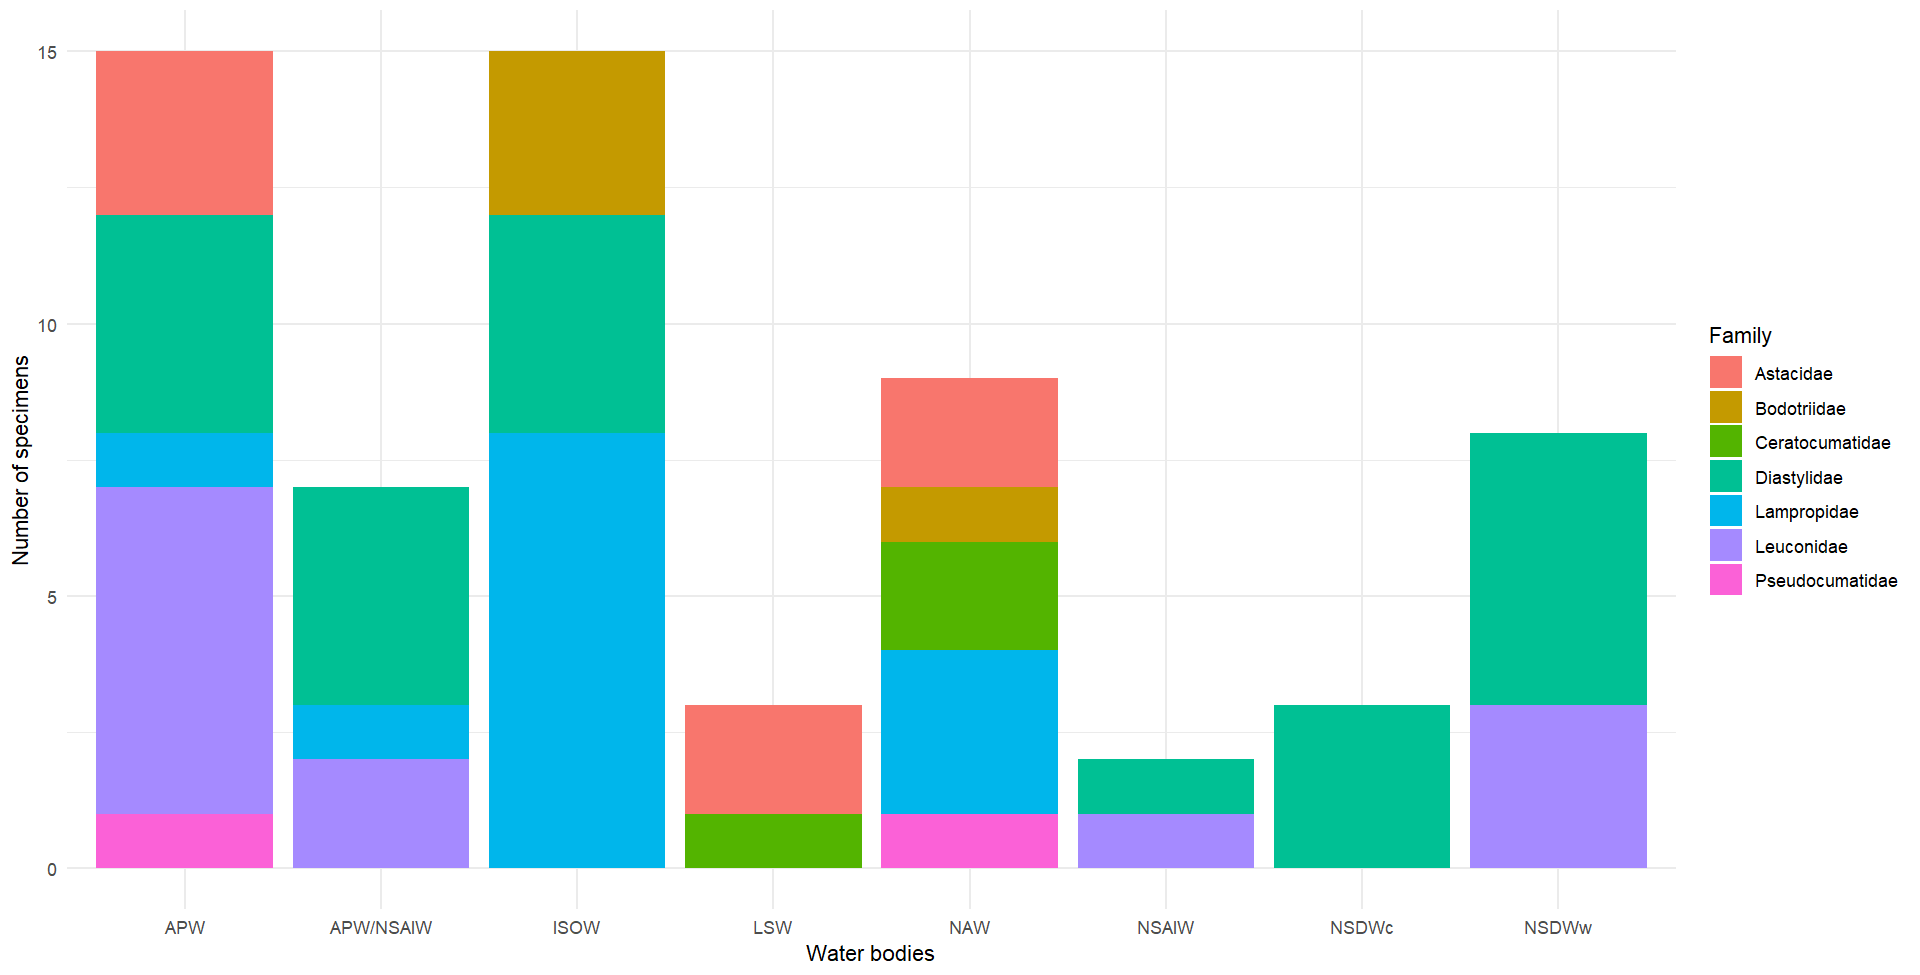
\includegraphics[width=0.7\textwidth]{figure3.png}
    \caption{Distribution of cumacean families by water mass. This histogram represents the frequency of occurrence of the various cumacean families in our samples, classified according to the body of water in which they were collected. Eight water mass categories are represented: APW (Arctic Polar Water), APW/NSAIW (Arctic Polar Water/North Sub-Arctic Intermediate Water), ISOW (Iceland Scotland Overflow Water), LSW (Labrador Sea Water), NAW (North Atlantic Water), NSAIW (North Sub-Arctic Intermediate Water), NSDWc (cold North Sub-Atlantic Deep Water), and NSDWw (warm North Sub-Atlantic Deep Water). Seven families are represented: Astacidae (red), Bodotriidae (brown), Ceratocumatidae (green), Diastylidae (turquoise), Lampropidae (blue), Leuconidae (purple), and Pseudocumatidae (pink). \label{fig:fig3}}
\end{figure}

The distribution of samples from different cumacean families according to the variety of water bodies where they were collected is illustrated in Figure \ref{fig:fig3}. This makes it possible to compare the diversity and potential preferences of the different families in each water mass, with the Diastylidae family being the most present in all the water masses (turquoise color). This testifies to the resistance and ecological adaptability of the Diastylidae family to a wide variety of environmental conditions, reminiscent of \emph{Leptostylis ampullacea} in Figure \ref{fig:fig2} which belongs to the Diastylidae family. Two water masses contain the greatest diversity of cumacean families, with APW (Arctic Polar Water) and NAW (North Atlantic Water) both having five families; APW: Astacidae, Diastylidae, Lampropidae, Leuconidae and Pseudocumatidae; NAW: Astacidae, Bodotriidae, Ceratocumatidae, Diastylidae, Lampropidae and Pseudocumatidae. This concomitance of different families could be explained by the diversified, resource-rich environments of these two water masses, supporting various complex ecological niches exploited by these families.

\begin{figure}[]
    \centering
    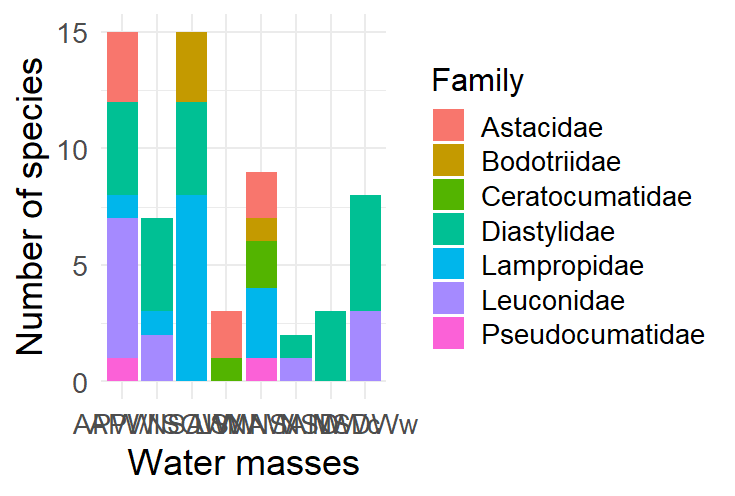
\includegraphics[width=0.7\textwidth]{figure4.png}
    \caption{Distribution of cumacean families by habitat. This histogram represents the frequency of occurrence of the different cumacean families in our samples, classified according to the type of habitat where they were collected. Three habitat categories are represented: Deep sea, Shelf, and Slope. Seven families are represented: Astacidae (red), Bodotriidae (brown), Ceratocumatidae (green), Diastylidae (turquoise), Lampropidae (blue), Leuconidae (purple), and Pseudocumatidae (pink). \label{fig:fig4}}
\end{figure}

The distribution of samples of the different families of cumacean according to the type of habitat where they were collected during sampling is shown in Figure \ref{fig:fig4}. This makes it possible to compare the diversity of different families in each habitat type. There is a wide variety of families in the deep sea providing different ecological niches, mainly dominated by the Diastylidae and the Lampropidae. The shelf also presents a variety of families, but less so than in the deep sea, with Leuconidae being the most abundant and acclimatized to these environmental conditions. The slope has the lowest diversity of the families, with a greater presence of Diastylidae, suggesting less varied ecological niches for cumaceans. The strong presence of families in particular habitats, such as the Diastylidae in the open sea and on the slope, and the Leuconidae on the continental shelf, suggests that these families have acquired adaptive characteristics (physiological, behavioral, or morphological), which could favor their survival in these specific environments. It also recommends that accessible resources (food and ecological niches) and environmental conditions, such as temperature, O\textsubscript{2} concentration, and sediment type, are essential factors in the distribution of cumacean families.

\begin{figure}[]
    \centering
    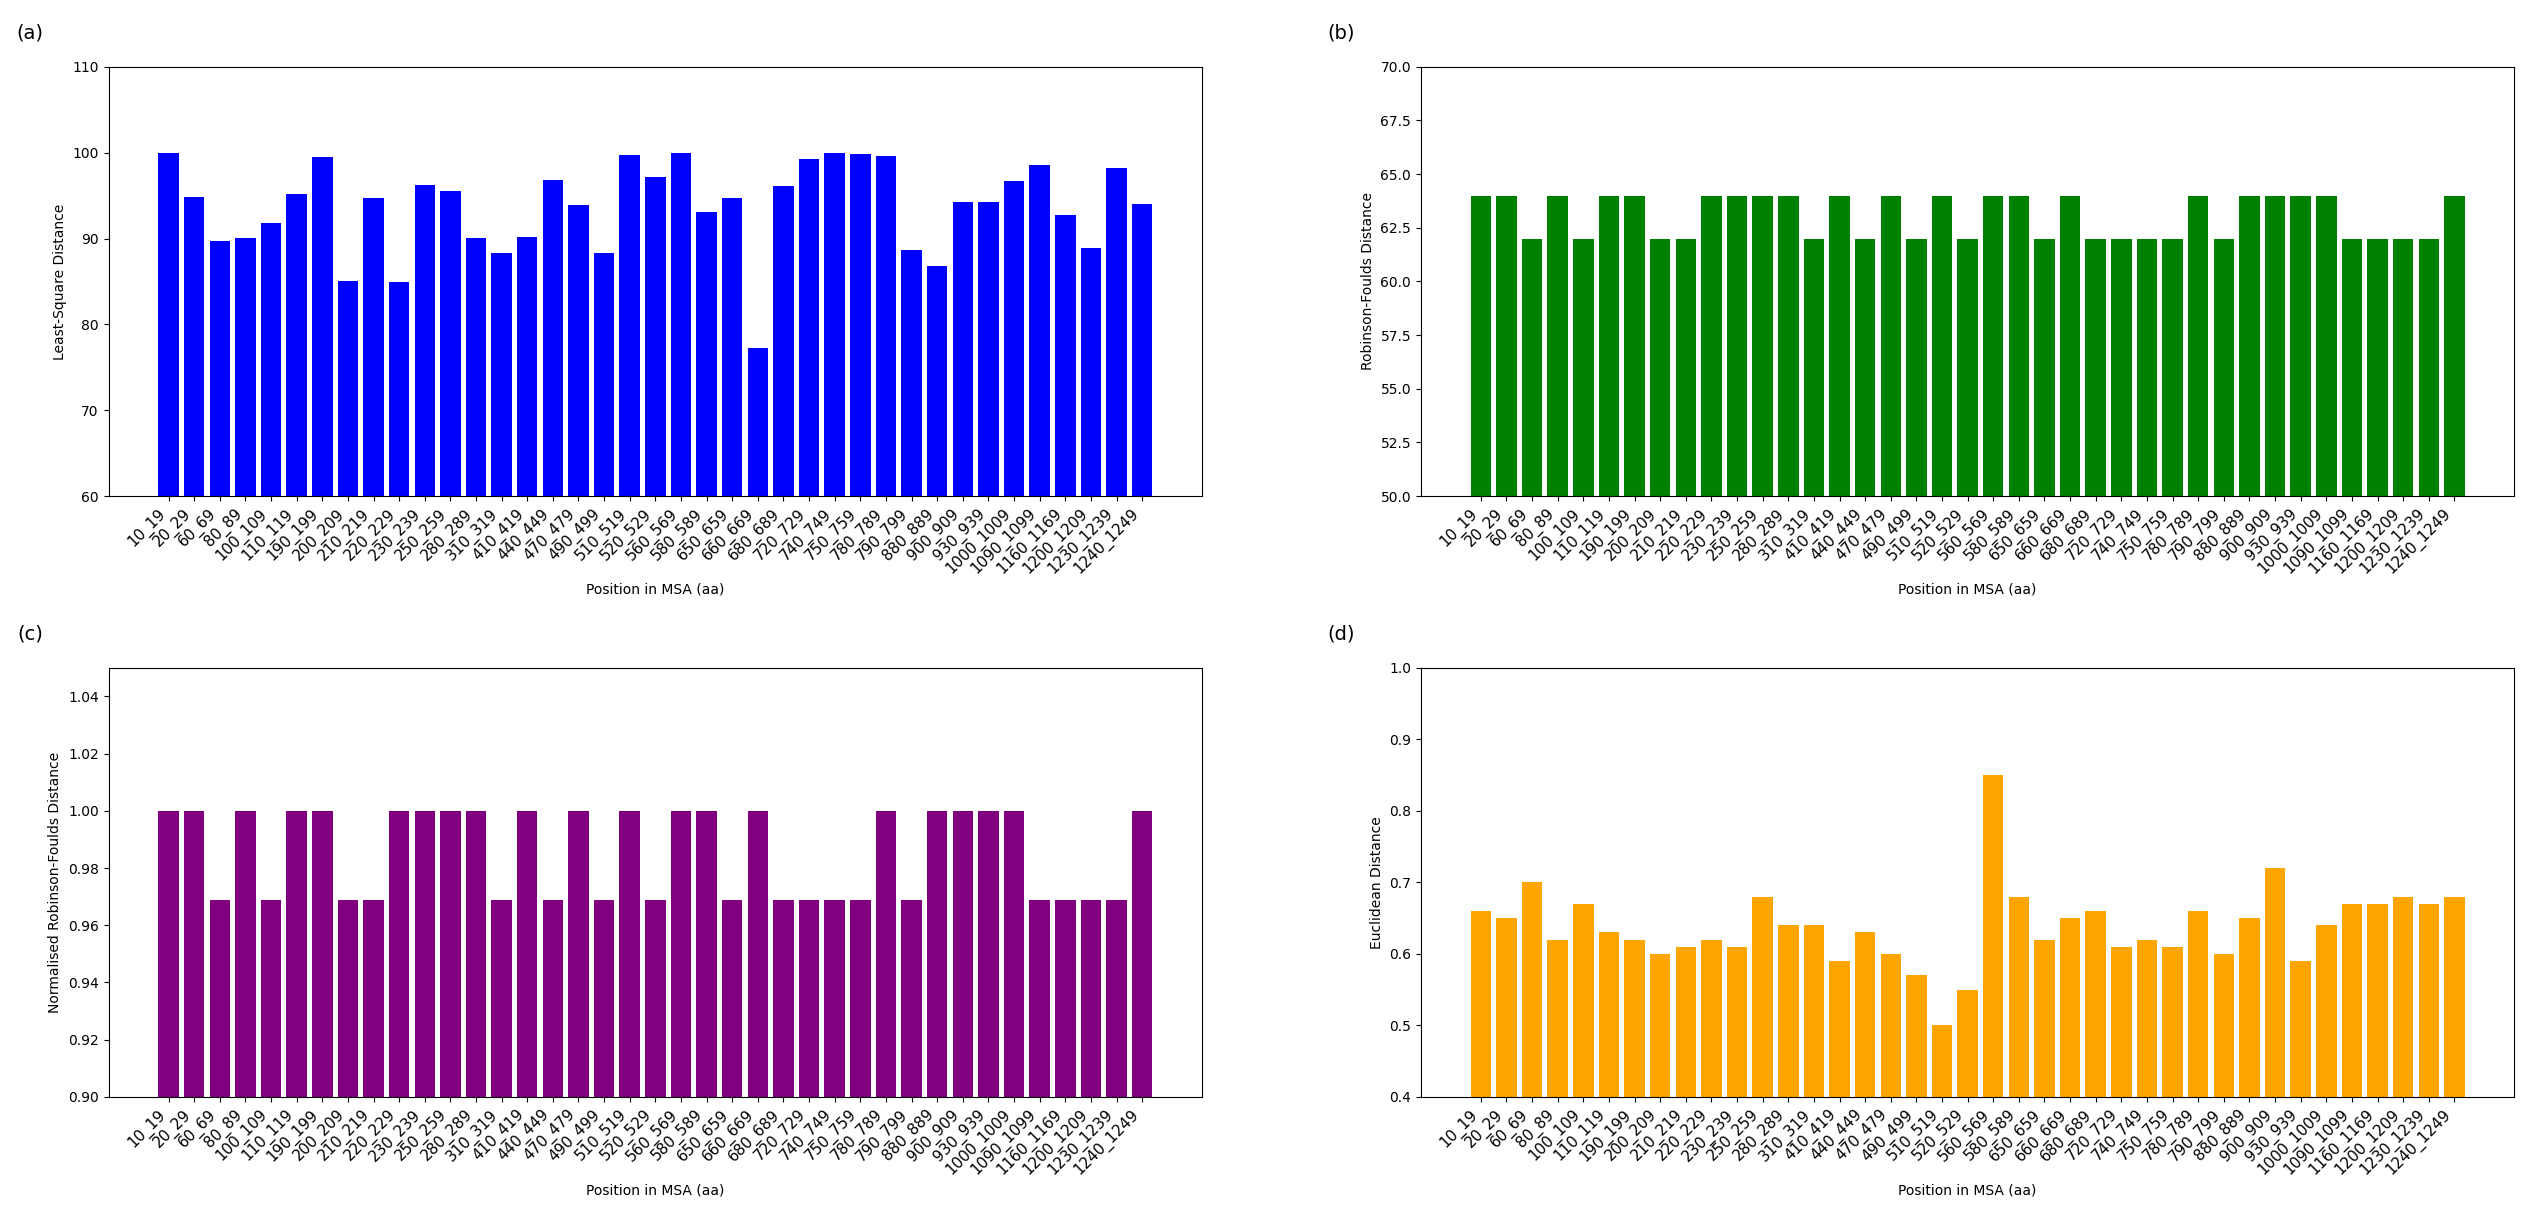
\includegraphics[width=0.7\textwidth]{figure5.png}
    \caption{Analysis of fluctuation in the four distance metrics using multiple sequence alignment (MSA): a) Least-Square distance, b) Robinson-Fouls distance, c) normalised Robinson-Fouls distance, and d) Euclidean distance. These distance variations are studied to establish their correlation with variation in wind speed (m/s) at the start of sampling. \label{fig:fig5}}
\end{figure}

\begin{figure}[]
    \centering
    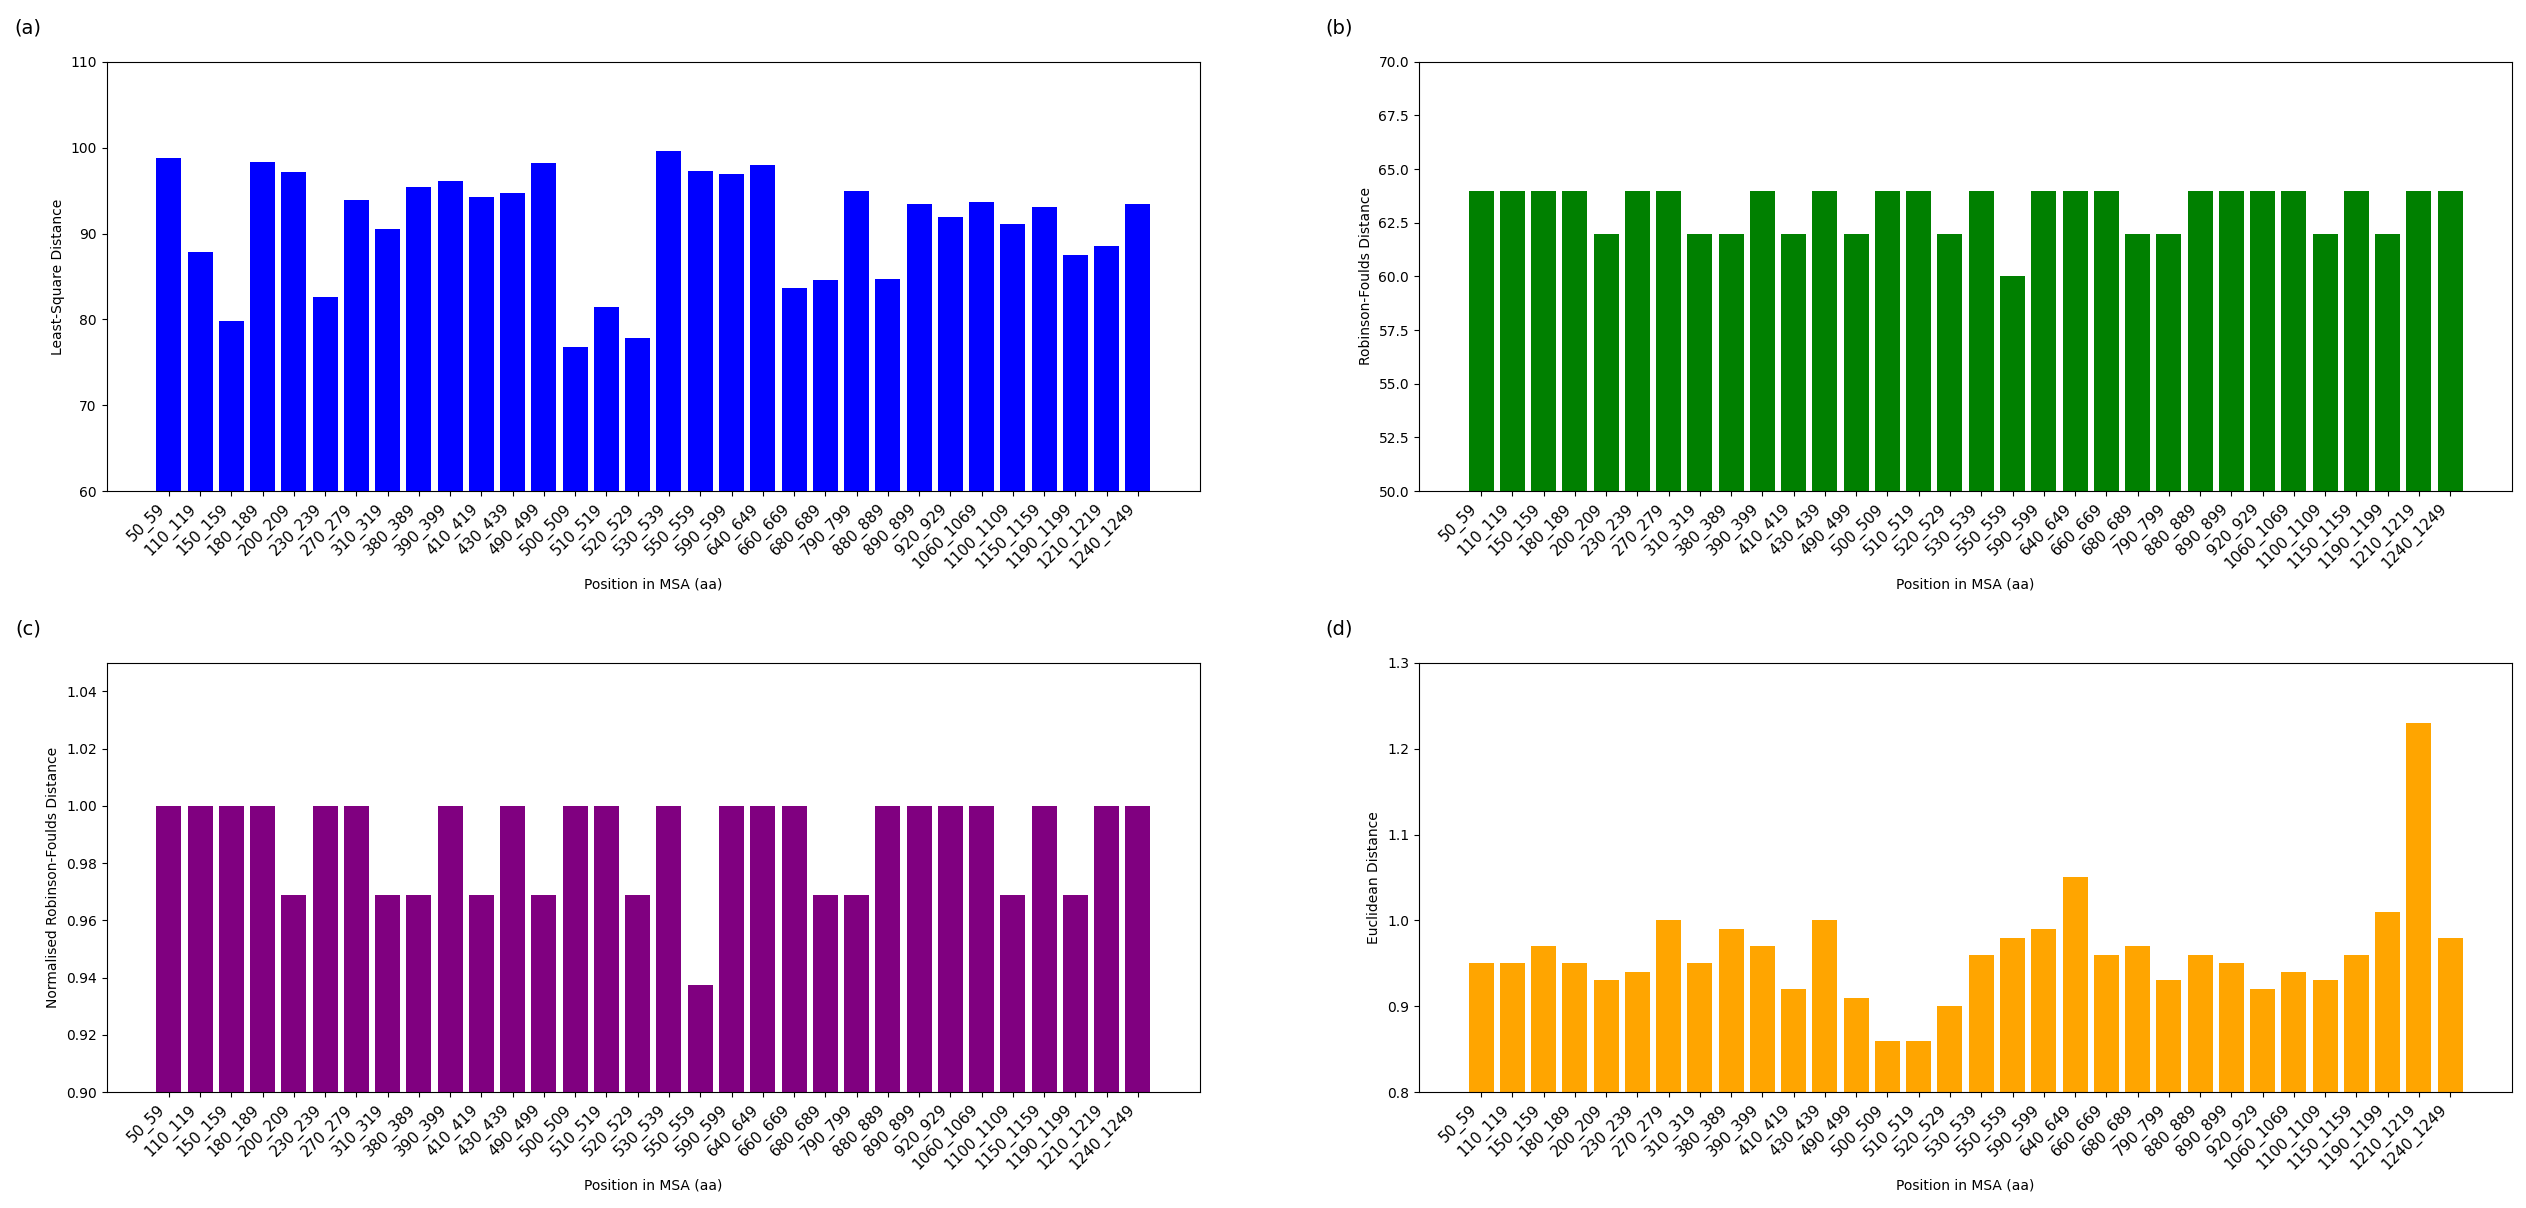
\includegraphics[width=0.7\textwidth]{figure6.png}
    \caption{Analysis of fluctuations in the four distance metrics using multiple sequence alignment (MSA): a) Least-Square distance, b) Robinson-Fouls distance, c) normalised Robinson-Fouls distance, and d) Euclidean distance. These distance variations are studied to establish their correlation with the variation in O\textsubscript{2} concentration (mg/L) where the samples were collected. \label{fig:fig6}}
\end{figure}

The correlation between genetic sequences and two attributes, one climatic (wind speed (m/s) at the start of sampling) and the other environmental (O\textsubscript{2} concentration (mg/L)) is presented in Figures \ref{fig:fig5} and \ref{fig:fig6}. These correlations are based on four metrics: Least Square Distance, Robinson-Fouls Distance, normalized Robinson-Foulds Distance, and Euclidean Distance. All the attributes presented in the first step of the \textit{aPhyloGeo} software section (see \textit{aPhyloGeo} software) were analyzed, but only these two parameters showed the most interesting mutation rate. Fluctuations in these parameters seem to reflect an adaptive response of these specific genetic sequences to environmental and climatic conditions. In both Figures, the Euclidean distance appears to be the most sensitive and heterogeneous from our data. A higher Euclidean distance means a greater difference between the sequences at positions 520 to 529 aa (see Figure \ref{fig:fig5}d) and 1190 to 1199 aa (see Figure \ref{fig:fig6}d), suggesting that these sites are more variable, subject to selection pressures or likely to change during evolution due to numerous mutations. 

All these results will need to be further investigated and analyzed to provide a more complete understanding of these results, and thus enable us to draw solid conclusions.

\section{Conclusion}\label{conclusion}

This study focuses on the effect of climatic, geographic, and environmental characteristics on cumacean genetics in the waters around Iceland. The main objective is to establish whether there is a correlation between the genetic information of the regions of the 16S rRNA mitochondrial gene (i.e. window) of cumacean species and the characteristics of their habitats. We aim to determine and identify the attribute most correlated with a specific genetic sequence and the associated protein. 

In this study, we selected relevant attributes from the IceAGE project data, BOLD Systems, and the article by \citep{uhlir_adding_2021}. We eliminated those that were not relevant to this study, as well as those that had low variance (e.g., salinity, $S^2 = 0.02146629$) or abundant missing data (> 95\%). Using these relevant data, we incorporated phylogeographic studies using the \textit{aPhyloGeo} software (see \autoref{lst:main}), in addition to the distribution analyses of certain attributes. The software makes it possible to examine potential correlations between the genetics of species and their environment, thus simplifying the interpretation of the evolution of species in various environmental contexts.

The results present variability in the cumacean environment according to the longitude (DD) at the start of sampling, the temperature ($^\circ$C) and  O\textsubscript{2} concentration of the water, and depth (m) at the beginning of sampling (see Figures \ref{fig:fig1}b, \ref{fig:fig1}e, \ref{fig:fig1}f and \ref{fig:fig1}c). Excluding wind speed (m/s) at the beginning of sampling (see Figure \ref{fig:fig1}d), violin diagrams present bimodal or multimodal curves, indicating the geographical and environmental separation of samples. DNA sequence analyses revealed specific genetic windows exposing high mutation rates in response to climatic and environmental attributes, such as wind speed (m/s) at the start of sampling and water O\textsubscript{2} concentration (mg/L) (see Figures \ref{fig:fig5}d and \ref{fig:fig6}d). The Euclidean distances of these two parameters showed fluctuation across the sequences, indicating sensitive or variable sites in evolution.

The results underline the importance of understanding the relationships between environmental, geographic, and climatic attributes and the genetics of benthic species such as cumacean. The correlations can be used to explain how these organisms acclimatize to climate change and anthropogenic disturbances, such as seabed mining. Therefore, our results can highlight conservation plans for regions sensitive to environmental and anthropogenic disturbance. For instance, the management of fishing and mining activities could use this knowledge to reduce their impact on benthic species. These notions are essential for the conservation of deep-sea ecosystems and for predicting the future impacts of environmental changes on marine biodiversity. In addition, this research can guide future studies on the genetic adaptation processes of cumacean to fluctuations in their ecoclimatic and geographic conditions.

However, further analysis is needed to examine these results in depth. It should be noted that we are missing three data of water O\textsubscript{2} concentration (mg/L) out of our 62 samples. This lack of data could impact the results as well as the final interpretations of this correlation. A complete study containing all the data would be required to certify these findings. In addition, this study is limited by the number of samples available ($n=62$), the methods used to assess genetic and environmental properties, and the logistical burden of data collection. To consolidate these results, it would be pertinent to study other species of invertebrates and other geographic regions. In particular, other relevant environmental, geographic, and climatic attributes should be investigated to better interpret genotype-environment interactions.


\section{Acknowledgments}\label{acknowledgments}

The authors thank the SciPy conference and reviewers for their valuable comments on this paper as well as Mansour Kebe for his technical support and Carolin Uhlir for her clarifications and advice on her study \citep{uhlir_adding_2021}. This work was supported by the Natural Sciences and Engineering Research Council of Canada (NSERC), the Fonds de recherche du Québec - Nature et technologies (FRQNT), the Université de Sherbrooke grant, and the Centre de recherche en écologie de l’Université de Sherbrooke (CREUS).

\appendix

\addcontentsline{toc}{section}{Supplementary material}

\section*{Supplementary material}

Figure \ref{fig:fig1} shows the variability of the dataset for two geographical (latitude and longitude at the start of sampling (DD)), one climatic (wind speed (m/s) at the start of sampling), and three environmental attributes (depth (m) at the start of sampling, temperature (°C) and the O\textsubscript{2}  concentration (mg/L) of the water). Violin diagrams display many of the same summary statistics as box plots: the white dots designate the medians, the thickened black bars in the center represent the interquartile range, and the thin black lines on either side evoke the rest of the distribution, except for the points that are rated as "extreme". On either side of the black lines is an approximation of the kernel density to show the shape of the data distribution. The wider areas of the violin diagrams show a higher probability of the variables taking a given value; the thinner areas indicate a lower probability. These diagrams are critical for designing the conditions of the habitats where the samples were collected, as high variability in the data may indicate heterogeneous habitats, while low variability indicates more homogeneous habitats. Thus, these violin plots allow to highlight unique habitats that can impact Cumacea genetics.

The mean, median, standard deviation, 1st and 3rd quartiles make it possible to identify general trends in the data, irregularities, or extreme values, and to capture the diversity of environmental conditions. Figure \ref{fig:fig1}a shows a latitude range at the start of sampling of 60.357 - 67.868 DD. The median of this distribution (67.15 DD) is higher than the mean (64.83 DD), indicating a skewed distribution towards lower values. This means that there are a few low values that drag the mean down. Unlike the mean, the median is less impacted by extreme values and provides an index of the central disposition of the data. The standard deviation (3.17 DD) shows a moderate dispersion close to the mean (64.83 DD). The quartiles Q1 (61.64 DD) and Q3 (67.64 DD) reveal that the majority of data are clustered around the median (67.15). The curve has an asymmetrical bimodal shape, showing two peaks, suggesting that the samples come from two dominant latitudinal regions at the start of sampling. This could indicate major fluctuations in climatic and environmental conditions in the regions sampled.  Similarly, this type of curve is present for the longitude (DD) at the start of sampling, as well as for the temperature (°C) and O\textsubscript{2} concentration (mg/L) of the water from which the samples were taken (see Figures \ref{fig:fig1}b,  \ref{fig:fig1}e and \ref{fig:fig1}f).

Figure \ref{fig:fig1}b shows a longitude distribution at the start of sampling from -31.356 - -12.162 DD. The median (-26.21 DD) is lower than the mean (-23.12 DD), suggesting an asymmetry on the side of higher values. This means that a few high values are pulling the mean upwards. The standard deviation (5.52 DD) indicates a relatively wide range of data. Quartiles Q1 (-26.77 DD) and Q3 (-18.14 DD) also show high variability in the longitude data at the start of sampling. This suggests a strong environmental gradient, geographical distribution and sample diversity from east to west in the region studied. 

Figure \ref{fig:fig1}c shows a depth range where samples were collected of 316 – 2568 m. The median (1574.70 m) is well above the mean (1412.57 m), showing an asymmetrical distribution towards the lower values. The standard deviation (881.16 m) is quite high, indicating significant variability in sample collection depths at the start of sampling and giving a more global overview of benthic habitats. Quartiles Q1 (579.10 m) and Q3 (2504.70 m) show and support, as does the standard deviation (881.16 m), a broad distribution of values. Important variations in standard deviation may indicate that some environmental parameters are more variable and could possibly impact Cumacea genetics differently. The curve of this figure has a multimodal shape with three prominent peaks, suggesting that the samples were mainly collected and concentrated at three different depths (around 500, 1500, and 2500 m).

Figure \ref{fig:fig1}d shows a range of wind speeds at the start of sampling from 2 – 11 m/s. The standard deviation (2.16 m/s) reveals a moderate spread of the data. Quartiles Q1 (5.25 m/s) and Q3 (7.00 m/s) suggest that most wind speeds fall within a fairly narrow distribution between 5.25 and 7.00 m/s. The mean (6.26 m/s) and median (6.00 m/s) are similar, with a high concentration of data around the median (6.00 m/s), indicating relatively stable wind conditions at the start of sampling.
Figure \ref{fig:fig1}e shows a temperature distribution where samples were collected from -0.851 - 4.28 $^\circ$C. The mean (1.45 $^\circ$C) is greater than the median (0.71 $^\circ$C), demonstrating an asymmetry towards higher values. The standard deviation (1.73 $^\circ$C) is relatively high compared to the mean (1.45 $^\circ$C), indicating a wide range of data. Quartiles Q1 (0.07 $^\circ$C) and Q3 (2.66 $^\circ$C) also show an expanded dispersion of water temperature values. These results suggest that water temperatures were very different depending on whether or not the sampling zones were close to the water surface, indicating acclimatization of cumaceans to a variety of habitat temperatures.

Figure \ref{fig:fig1}f shows a range of O\textsubscript{2} concentration in the water where the samples were collected from 245.53 - 292.97 mg/L. The median (278.77 mg/L) is higher than the mean (271.88 mg/L), showing an asymmetry towards the lower values. Quartiles Q1 (258.39 mg/L) and Q3 (290.90 mg/L) show some variability in the O\textsubscript{2} concentration data, also supported by the standard deviation (18.11 mg/L). These latest results reflect a diversity of O\textsubscript{2}  requirements, with organisms adapted to low O\textsubscript{2} conditions and potentially influenced by the heterogeneity of biogeochemical cycles, such as photosynthesis, respiration, and organic decomposition, which impact dissolved O\textsubscript{2} levels as a function of depth.

The distribution and diversity of the different cumacean species found in our sample are presented in Figure \ref{fig:fig2}. It helps in visualizing the most represented species (\emph{Leptostylis ampullacea}, 14.1\%; \emph{Leucon pallidus}, 12.5\%) and the less represented species (\emph{Bathycuma brevirostre}, \emph{Leucon spinulosus}, \emph{Styloptocuma gracillimum}, \emph{Campylaspis horrida}, \emph{Campylaspis globosa}, and \emph{Hemilamprops uniplicatus}; all 1.6\%). suggesting variations in sampling, particular ecological forces that favor or limit certain species, or that certain species have a restricted ecological niche. In contrast to the lesser represented species, dominant species may have particular adaptive traits that contribute to their exploitation of food, their interspecific competition, or their resistance to changing environmental conditions.

Comparing each species’ frequency with the mean and median (see top right-hand corner of Figure \ref{fig:fig2}) also helps to identify which species are more or less frequent. As mentioned above, \emph{Leptostylis ampullacea} and \emph{Leucon pallidus}, with above-average frequencies, are dominant species. Thus, the presence of species with frequencies higher or lower than the mean (2.00) and median (2.85) amplified variations in sampling or particular ecological forces that advantage or disadvantage certain species. Furthermore, a median (2.00) lower than the mean (2.85) indicates that most species have relatively low frequencies, while there are a few species with higher frequencies, indicating an asymmetrical distribution.

The distribution of samples from different cumacean families according to the variety of water bodies where they were collected is illustrated in Figure \ref{fig:fig3}. This makes it possible to compare the diversity and potential preferences of the different families in each body of water.

APW (Arctic Polar Water) has a high family diversity, with a significant presence of the Leuconidae, Diastylidae, and Astacidae. APW/NSAIW (Arctic Polar Water/North Sub-Arctic Intermediate Water) shows a high presence of Diastylidae and Leuconidae, with a low density of Lampropidae. ISOW (Iceland Scotland Overflow Water) has a great abundance of specimens, including Lampropidae and Diastylidae. LSW (Labrador Sea Water) shows low family diversity, with a preponderance of Astacidae. NAW (North Atlantic Water), like APW (Arctic Polar Water), has a high family diversity, with a predominance of Lampropidae, Ceratocumatidae, and Astacidae. NSAIW (North Sub-Arctic Intermediate Water) shows, like LSW (Labrador Sea Water), a low family diversity, represented by the Leuconidae and the Lampropidae. NSWc and NSDWw (North Sub-Atlantic Deep Water, cold and warm), have high abundances of Diastylidae, with the presence of Leuconidae in NSDWw (warm North Sub-Atlantic Deep Water).

This testifies to the resistance and ecological adaptability of the Diastylidae family to a wide variety of environmental conditions, reminiscent of \emph{Leptostylis ampullacea} in Figure \ref{fig:fig2} which belongs to the Diastylidae family. Two water masses contain the greatest diversity of cumacean families, with APW (Arctic Polar Water) and NAW (North Atlantic Water) both having five families; APW: Astacidae, Diastylidae, Lampropidae, Leuconidae and Pseudocumatidae; NAW: Astacidae, Bodotriidae, Ceratocumatidae, Diastylidae, Lampropidae and Pseudocumatidae. This concomitance of different families could be explained by the diversified, resource-rich environments of these two water masses, supporting various complex ecological niches exploited by these families.

The distribution of samples of the different families of cumacean according to the type of habitat where they were collected during sampling is shown in Figure \ref{fig:fig4} . This makes it possible to compare the diversity of different families in each habitat type.

Deep sea, there is a wide variety of families, dominated by the Diastylidae and the Lampropidae. Shelf presents a wide variety of families, but less than the deep sea. It is dominated by the Leuconidae. Slope, shows low family diversity, with a greater presence of Diastylidae. 

The strong presence of families in particular habitats, such as the Diastylidae in the open sea and on the slope, and the Leuconidae on the continental shelf, suggests that these families have acquired adaptive characteristics (physiological, behavioral, or morphological), which could favor their survival in these specific environments. It also recommends that accessible resources (food and ecological niches) and environmental conditions, such as temperature, O\textsubscript{2} concentration, and sediment type, are essential factors in the distribution of cumacean families.

The correlation between genetic sequences and two attributes, one climatic (wind speed (m/s) at the start of sampling) and the other environmental (O\textsubscript{2}  concentration (mg/L)) is presented in Figures \ref{fig:fig5} and \ref{fig:fig6}. This correlation was based on four metrics: Least-Square Distance, Robinson-Fouls Distance, Normalised Robinson-Foulds Distance, and Euclidean Distance.  All the attributes presented in the first step of the \textit{aPhyloGeo} software section (see \textit{aPhyloGeo} software) were analyzed, but only these two parameters showed the most interesting mutation rate. Fluctuations in these parameters seem to reflect an adaptive response of these specific genetic sequences to environmental and climatic conditions. 

Sequence correlation raises the question of how variations in sequences (i.e., windows) respond to or vary with climatic and environmental conditions. Conserved positions (low values) could potentially suggest functionally essential regions that do not readily vary with changing conditions. On the other hand, fluctuating positions (high values) could present specific adaptations to conditions, in this case climatic and environmental. Analyzing how sequences do or do not vary under these two different conditions can highlight regions in the sequences (i.e., windows) that are sensitive or resistant to fluctuations in these two attributes. In our results, we observe a similar fluctuation of the correlation with these two parameters between Figures \ref{fig:fig5} and \ref{fig:fig6}.

In Figure \ref{fig:fig5}a, the peaks and troughs suggest that some locations across the sample sequences are more conserved and therefore similar (smaller distance), probably indicating potential functional or structural significance, while other positions show more variability (larger distance). In contrast to Figure \ref{fig:fig5}a, the values in Figure \ref{fig:fig5}b are more concentrated on restricted values, suggesting a more uniform fluctuation. In this context, lower variation may indicate that changes in sequences do not completely affect local phylogeny. The same is true of Figure \ref{fig:fig5}c, where the normalized distances are rather homogeneous, dictating that variations in sequence positions have a fairly constant impact on the phylogenic structure of the trees. The Euclidean distance, shown in Figure \ref{fig:fig5}d, appears to be the most sensitive and disparate distance to our data. A higher Euclidean distance means a greater difference between sequences at position 520 aa to 529 aa, suggesting that this site is more variable or evolutionarily susceptible to change.

Figure \ref{fig:fig6}a is similar to Figure \ref{fig:fig5}a but shows more variation between different window positions. Windows with smaller mean-squared distances are more likely to be evolutionarily conserved, while windows with larger distances show greater instability. The Robinson-Foulds distances in Figure \ref{fig:fig6}b vary with a restricted range of values (50 to 70). These small variations suggest that fluctuations in sequences do not significantly alter local phylogeny. Like the figure above, Figure \ref{fig:fig6}c has a fairly homogeneous distribution. This means that variations in individual window positions exert a fairly uniform influence on the phylogenetic arrangement of trees following normalization. Like Figure \ref{fig:fig5}d, the Euclidean distance presented in Figure \ref{fig:fig6}d shows the greatest sensitivity and heterogeneity from our data. The position with the highest Euclidean distance (between 1190 aa to 1199 aa) shows significant dissimilarity between sequences at this position, which may signify a more fluctuating or evolutionarily unstable site due to numerous mutations.

